\chapter{Sorption}\label{appSec:Sorption} 

\begin{table}
\caption{Freundlich sorption coefficients and standard errors for isotherms. $log~K_F$ for the soil samples are the collective partition coefficients for soil and biochar because. All $K_F$ data are in units of $\mathrm{(\mu g/kg)/(\mu g/L)^{n_F}}$.}
\centering
\adjustbox{max width=\textwidth}{%
\begin{threeparttable}
\label{apptab:summary_stats_all}
\begin{tabular}{lllllllll} \toprule
\multicolumn{1}{c}{Compound} & \multicolumn{1}{c}{Biochar} & \multicolumn{1}{c}{type} & \multicolumn{1}{c}{$log~K_F$} & \multicolumn{1}{c}{se $log~K_F$} & \multicolumn{1}{c}{$n_F$} & \multicolumn{1}{c}{se $n_F$} & \multicolumn{1}{c}{$r^2$} & \multicolumn{1}{c}{$p$} \\ \midrule
PFPeA & CWC & BC\_S\_mix & \multicolumn{1}{c}{\textbf{}} & \multicolumn{1}{c}{\textbf{}} & \multicolumn{1}{c}{\textbf{}} & \multicolumn{1}{c}{\textbf{}} & \multicolumn{1}{c}{\textbf{}} & \multicolumn{1}{c}{\textbf{}} \\
PFHxA & CWC & BC\_S\_mix & 3.05 & 0.95 & 0.61 & 0.39 & 0.38 & \textgreater{}0.05 \\
PFHpA & CWC & BC\_S\_mix & 3.30 & 0.23 & 0.46 & 0.14 & 0.73 & * \\
PFOA & CWC & BC\_S\_mix & 3.25 & 0.48 & 0.77 & 0.18 & 0.82 & * \\
PFNA & CWC & BC\_S\_mix & 3.84 & 0.28 & 0.60 & 0.10 & 0.89 & * \\
PFDA & CWC & BC\_S\_mix & 4.31 & 0.18 & 0.57 & 0.06 & 0.95 & ** \\
PFOA & CWC & BC\_S\_sing & 3.45 & 0.21 & 0.88 & 0.09 & 0.96 & ** \\
PFPeA & CWC & BC\_sing & 3.98 & 0.36 & 0.56 & 0.33 & 0.30 & \textgreater{}0.05 \\
PFHxA & CWC & BC\_sing & 4.59 & 0.50 & -0.14 & 0.26 & 0.04 & \textgreater{}0.05 \\
PFHpA & CWC & BC\_sing & 4.44 & 0.05 & 0.59 & 0.11 & 0.80 & ** \\
PFOA & CWC & BC\_sing & 5.06 & 0.08 & 0.39 & 0.05 & 0.90 & *** \\
PFNA & CWC & BC\_sing & 4.88 & 0.04 & 0.65 & 0.04 & 0.98 & *** \\
PFDA & CWC & BC\_sing & 5.22 & 0.07 & 0.45 & 0.04 & 0.94 & *** \\
\addlinespace
PFPeA & DSL & BC\_S\_mix &  &  &  &  &  &  \\
PFHxA & DSL & BC\_S\_mix & 4.54 & 0.30 & 0.18 & 0.15 & 0.33 & \textgreater{}0.05 \\
PFHpA & DSL & BC\_S\_mix & 4.10 & 0.19 & 0.09 & 0.15 & 0.10 & \textgreater{}0.05 \\
PFOA & DSL & BC\_S\_mix & 4.91 & 0.06 & 0.39 & 0.03 & 0.97 & *** \\
PFNA & DSL & BC\_S\_mix & 5.10 & 0.06 & 0.35 & 0.03 & 0.97 & *** \\
PFDA & DSL & BC\_S\_mix & 5.48 & 0.04 & 0.35 & 0.03 & 0.98 & *** \\
PFOA & DSL & BC\_S\_sing & 5.08 & 0.10 & 0.46 & 0.08 & 0.90 & * \\
PFPeA & DSL & BC\_sing & 4.25 & 0.74 & 0.14 & 0.38 & 0.06 & \textgreater{}0.05 \\
PFHxA & DSL & BC\_sing & 3.30 & 0.15 & 1.12 & 0.11 & 0.93 & *** \\
PFHpA & DSL & BC\_sing & 4.67 & 0.06 & 0.57 & 0.09 & 0.86 & *** \\
PFOA & DSL & BC\_sing & 5.12 & 0.02 & 0.60 & 0.02 & 0.99 & *** \\
PFNA & DSL & BC\_sing & 5.33 & 0.03 & 0.80 & 0.07 & 0.94 & *** \\
PFDA & DSL & BC\_sing & 5.61 & 0.02 & 0.61 & 0.02 & 0.99 & *** \\
\addlinespace 
PFPeA & ULS & BC\_S\_mix &  &  &  &  &  &  \\
PFHxA & ULS & BC\_S\_mix & 4.39 & 0.13 & 0.32 & 0.06 & 0.86 & ** \\
PFHpA & ULS & BC\_S\_mix & 4.12 & 0.13 & 0.14 & 0.10 & 0.35 & \textgreater{}0.05 \\
PFOA & ULS & BC\_S\_mix & 5.00 & 0.05 & 0.39 & 0.03 & 0.98 & *** \\
PFNA & ULS & BC\_S\_mix & 5.22 & 0.04 & 0.37 & 0.03 & 0.97 & *** \\
PFDA & ULS & BC\_S\_mix & 5.62 & 0.04 & 0.37 & 0.03 & 0.97 & *** \\
PFOA & ULS & BC\_S\_sing & 5.16 & 0.03 & 0.62 & 0.03 & 0.99 & *** \\
PFPeA & ULS & BC\_sing & 4.10 & 0.13 & 0.67 & 0.16 & 0.74 & ** \\
PFHxA & ULS & BC\_sing & 4.80 & 0.06 & 0.34 & 0.09 & 0.72 & ** \\
PFHpA & ULS & BC\_sing & 5.98 & 0.17 & 1.08 & 0.11 & 0.93 & *** \\
PFOA & ULS & BC\_sing & 5.73 & 0.02 & 0.65 & 0.05 & 0.95 & *** \\
PFNA & ULS & BC\_sing & 5.89 & 0.02 & 0.71 & 0.03 & 0.99 & *** \\
PFDA & ULS & BC\_sing & 6.00 & 0.04 & 0.35 & 0.05 & 0.86 & *** \\ \bottomrule
\end{tabular}
\begin{tablenotes}
\item Significant codes: *** $\sim$ 0.001, ** $\sim$ 0.01, * $\sim$ 0.05
\end{tablenotes}
\end{threeparttable}}
\end{table}


\section{Alternative sorption mechanism explanation}
Give short intro 

\begin{figure}[htb]
    \centering
    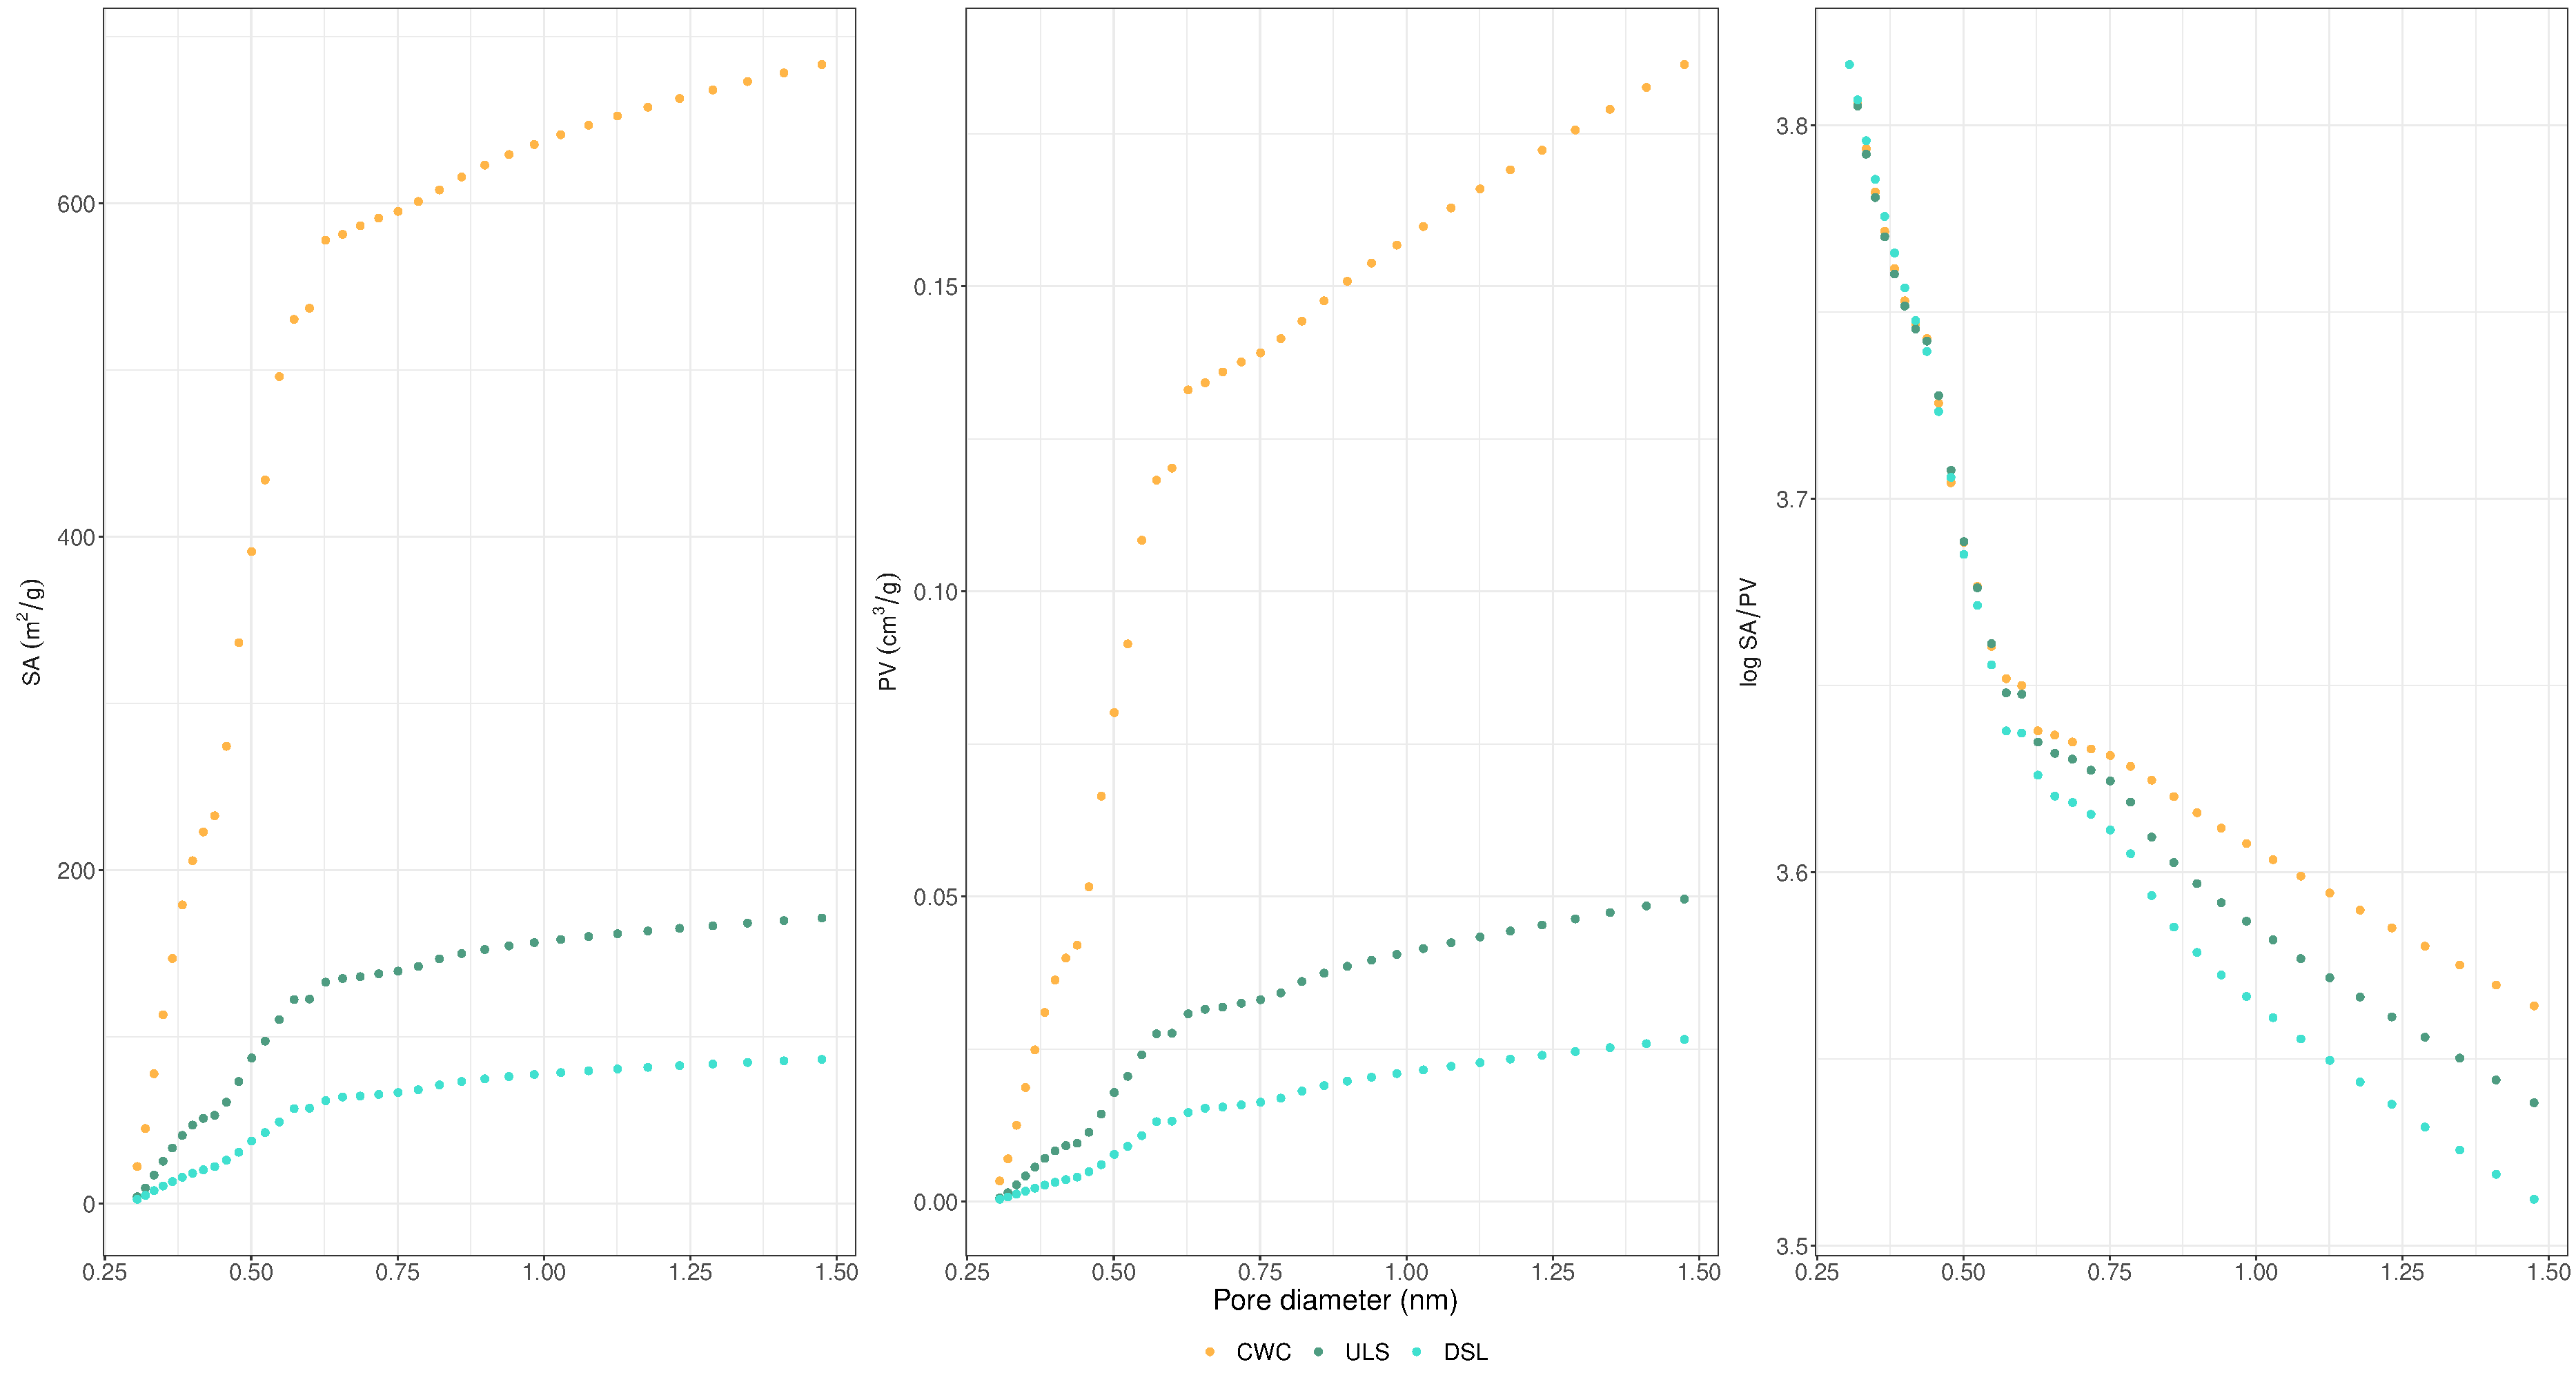
\includegraphics[width=\textwidth]{R/figs/PZD_appendix_small.pdf}
    \caption{Cumulative pore size distribution for pores 0.4-1.5 nm using DFT with (a) surface area (SA), (b) pore volume (PV), and (c) SA/PV ratio.}
    \label{appfig:PZD_small}
\end{figure}

\begin{figure}[htb]
    \centering
    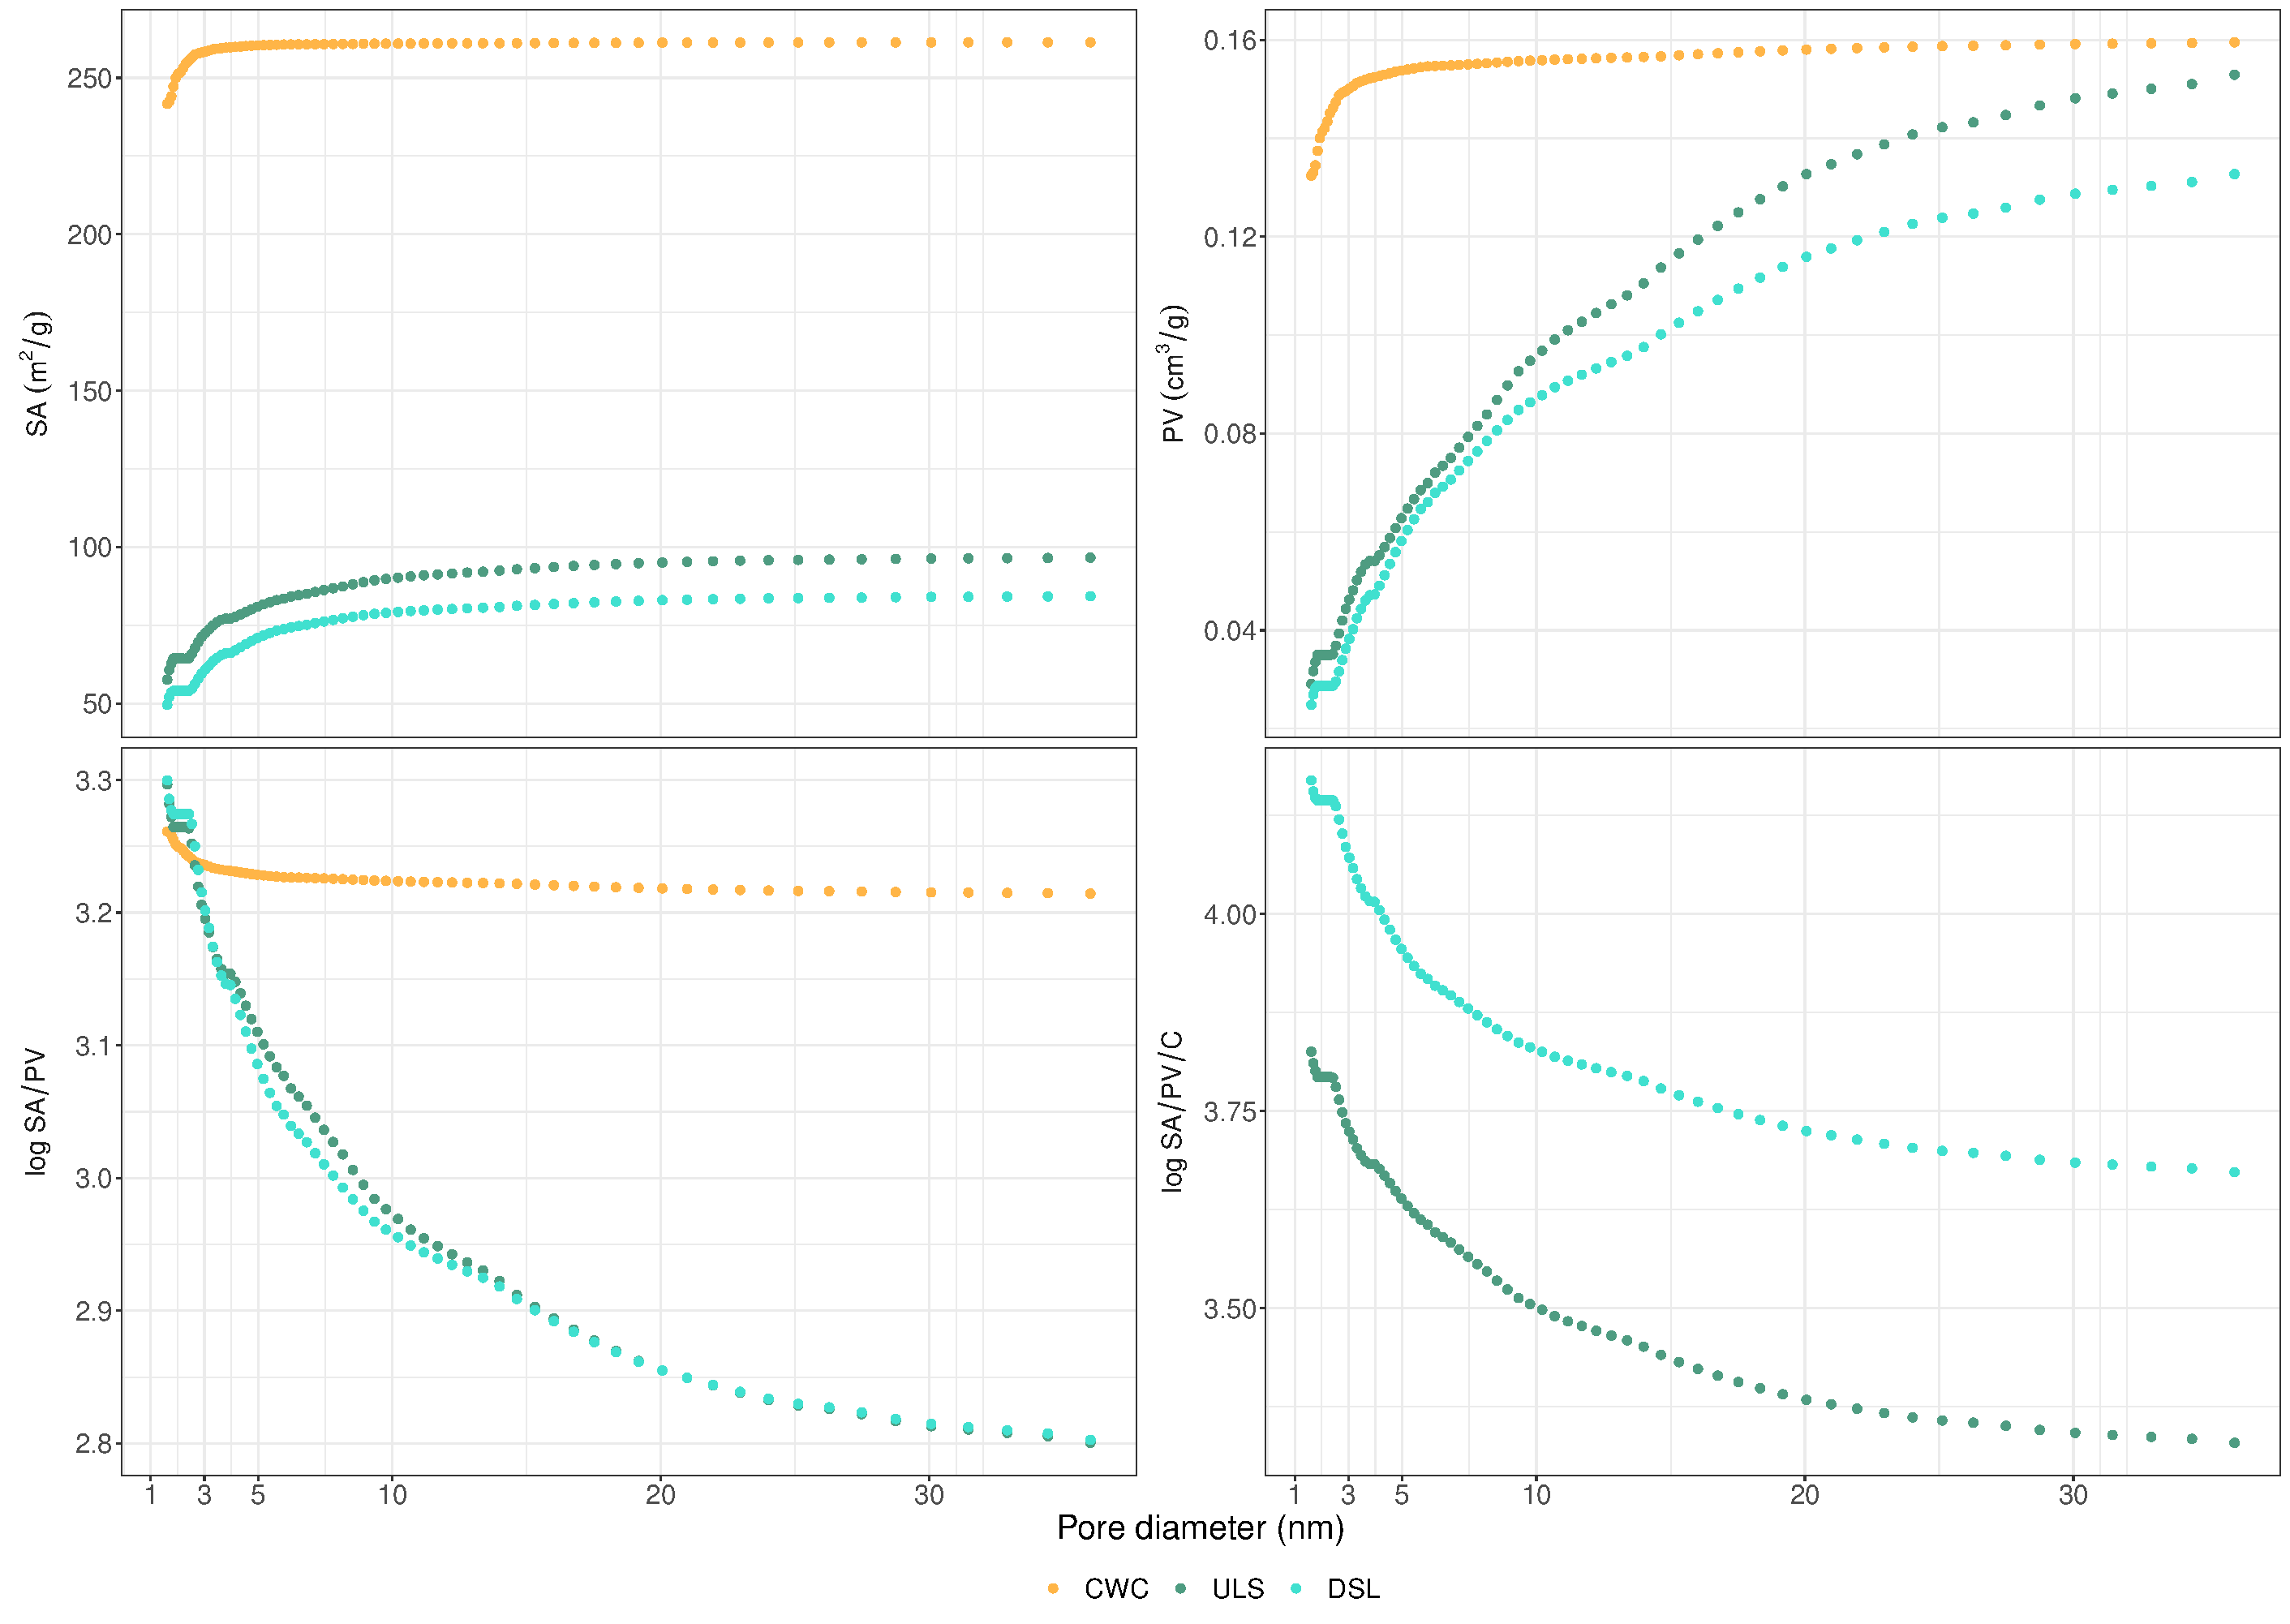
\includegraphics[width=\textwidth]{R/figs/PSD_appendix_large.pdf}
    \caption{Cumulative pore size distribution for pores $>$ 1.5 nm using DFT theory with (a) surface area (SA) and (b) pore volume (PV), (c) log SA/PV, (d) log SA/PV/C (carbon).}
    \label{appfig:PZD_large}
\end{figure}

\begin{table}
\centering
\caption{Surface area (SA), pore volume (PV), elemental content (C, O, H, N) and ratios for the biochars produced for the batch tests.}
\adjustbox{max width=\textwidth}{
\label{apptab:SAPV}
\begin{tabular}{llrrrrrrlllllll}
\toprule
Biochar & \multicolumn{4}{l}{N\textsubscript{2} sorption} & \multicolumn{3}{l}{CO\textsubscript{2} sorption} & \multicolumn{4}{c}{Elemental content} & \multicolumn{3}{c}{Elemental ratio} \\
sorbent & \multicolumn{4}{l}{(pores \textgreater 1.5 nm)} & \multicolumn{3}{l}{(pores 0.4-1.5 nm)} & & & & & & \\ \cmidrule(l){2-5} \cmidrule(l){6-8} \cmidrule(l){9-12} \cmidrule(l){13-15} 
& BET SA  & BJH PV & log SA/PV & log SA/PV/C & DFT SA & DFT PV & log SA/PV & C & O & H & N & O/C & H/C & N/C \\
& ($\mathrm{m^2~g^{-1}}$) & (cm\textsuperscript{3} g\textsuperscript{-1}) & ($\mathrm{m^2 cm^{-3}}$) & ($\mathrm{m^2 cm^{-3} g^{-1}}$)& ($\mathrm{m^2~g^{-1}}$) & (cm\textsuperscript{3} g\textsuperscript{-1}) & ($\mathrm{m^2 cm^{-3}}$) & (\%) & (\%) & (\%) & (\%) & & & \\ \midrule
CWC & 323 & 0.017 & 4.28 & 2.32 & 683 & 0.186 & 3.54 & 91.4 & 5.50 & 1.01 & 0.69 & 0.06 & 0.01 & 0.008       \\
ULS & 128 & 0.126 & 3.01 & 1.54 & 165 & 0.047 & 3.57 & 29.6 & 57.1 & 1.24 & 1.13 & 1.9  & 0.04 & 0.04        \\
DSL & 110 & 0.111 & 3.00 & 1.87 & 87  & 0.027 & 3.51 & 13.5 & 61.4 & 1.05 & 0.82 & 4.6  & 0.08 & 0.06       \\ \bottomrule
\end{tabular}}
\end{table}

The surface area to pore volume ratio (SA/PV) can be used to more accurately represent available sorption sites, where a lower ratio indicates higher porosity \citep{presser2011SAPV}. Since PV increases by increasing pore diameter (\cref{appfig:PZD_small}), the relative increase in PV will be higher than the relative increase in SA. This means that the SA/PV ratio is expected to decrease more rapidly for biochar with higher pore volumes. This expectation is confirmed in \cref{fig:PZD_small} where the SA/PV ratios for ULS and DSL are nearly equivalent to CWC, despite the fact that SA and PV are significantly different from CWC taken separately. This is reflected in the cumulative SA/PV ratios (\cref{tab:SAPV}) which are similar: 3 674, 3 502, and 3 206 m\textsuperscript{2} cm\textsuperscript{-3} for CWC, ULS, and DSL respectively. This means that despite CWC being more numerous in micropores than ULS and DSL, its porosity is similar, and is predominantly allocated within the ultra micropore fraction.

Similar to the trend for small pores, CWC also had the largest cumulative SA but the lowest PV for pores $>$1.5 nm (323 m\textsuperscript{2} g\textsuperscript{-1} versus 110 and 128 m\textsuperscript{2} g\textsuperscript{-1} for DSL and ULS, respectively). \cref{appfig:PZD_large}a shows that the highest proportion of SA is allocated to pores between 1.5-3 nm for CWC and 1.5-5 nm for ULS and DSL. Cumulative PV is highest for ULS (0.126 cm\textsuperscript{3} g\textsuperscript{-1}), where PV for CWC was one order of magnitude lower (0.017 cm\textsuperscript{3} g\textsuperscript{-1}). Furthermore, the development of PV with pore diameter in \cref{fig:PZD_large}b shows a clear distinction between CWC and the two sewage sludge biochars. CWC has most of its PV in pores $<$3 nm, whereas PV for ULS and DSL steadily increase up to the maximum pore size of 35 nm. This difference becomes important for the SA/PV ratio seen in \cref{fig:PZD_large}c. Here, ULS and DSL have low and equivalent cumulative $\log~SA/PV$ ratios of 2.8 compared to the higher ratio of 3.2 for CWC (\cref{tab:SAPV}). Previous studies have consistently concluded that a large internal surface area and pore volume of adsorbents are the two most important parameters for achieving high sorption capacity of PFAS \citep{du2014adsorption,Sormo2021,Hale2016,ahmed2020per}. Similarly, the results of this study provide clear indications that a low SA/PV ratio can be considered a proxy for good PFAS sorption. The most plausible explanation for why CWC is the weakest sorbent among the three samples in this study is that CWC consists almost exclusively of micropores, whereas ULS and DSL also have pores in the mesopore range (2-50 nm). The shift observed by comparing SA and PV together demonstrates the importance of considering both pore size \textit{and} surface area when evaluating available sorption sites on biochar.

Since ULS and DSL had nearly equivalent SA/PV ratios, an additional parameter is needed to explain why ULS is a better sorbent than DSL (\cref{fig:PZD_large}c). Apart from SA and PV, carbon content has, in previous literature, been a good predictor of sorption affinity to PFAS \citep{Hale2016,Cornelissen2005}. ULS contains 29.6 \% carbon whereas DSL contains 13.5 \%. This means that high porosity and sufficiently large pores are the two most important parameters that regulate high sorption capacity, and that the pore wall composition further contributes to enhanced sorption. 

\Cref{appfig:Kd_SAPV_C} shows the relationship between each of carbon content ($\log~C$), $\log~SA/PV$ and $\log~SA/PV/C$, now as a function of $\log~K_d$ (normalized to 1 $\mu g~L^{-1}$). This figure shows that a linear relationship exists between $\log~K_d$ and $\log~SA/PV/C$, and that no such relationship is present for carbon content and the SA/PV ratio individually. 

\begin{figure}[htb]
    \centering
    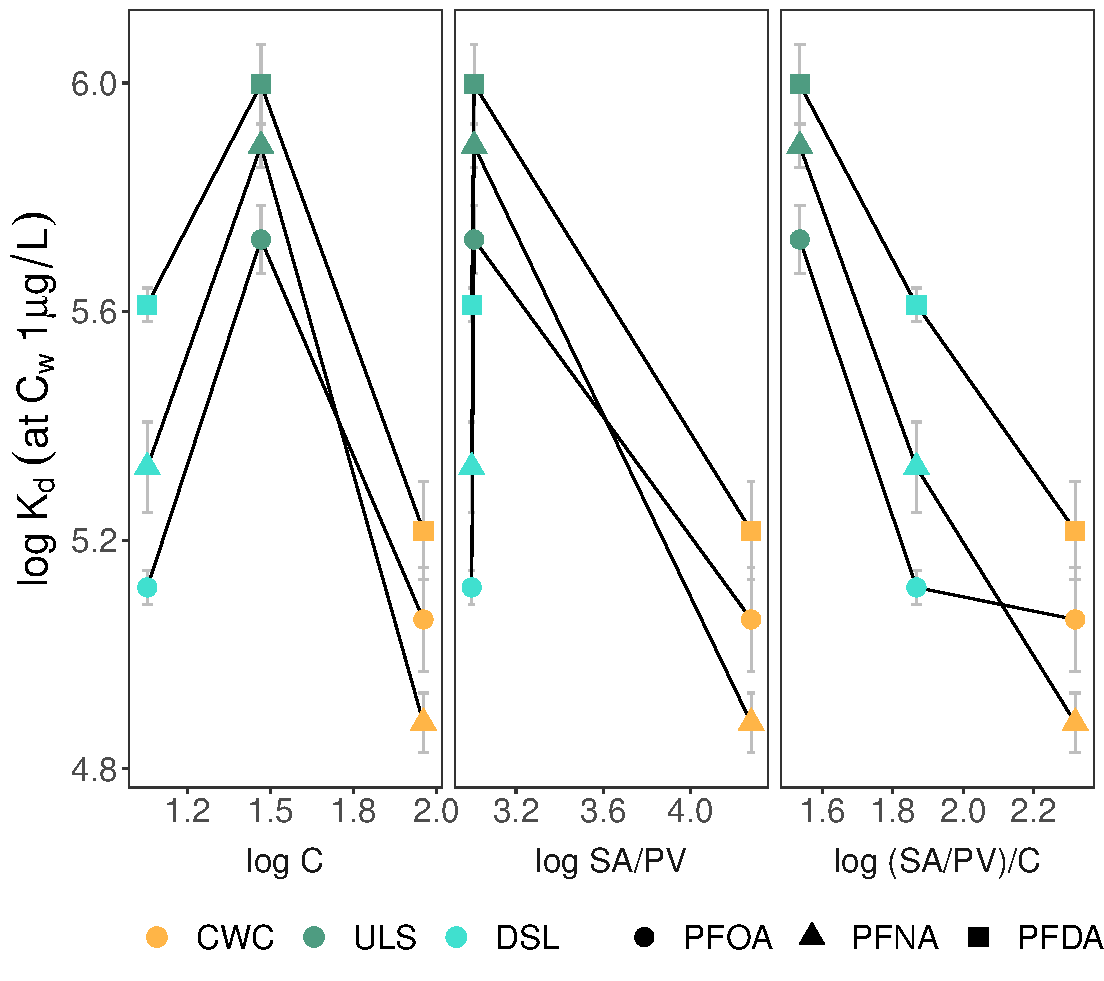
\includegraphics[width=0.8\textwidth]{R/figs/SAPV_C_Kd1ugL_plot.pdf}
    \caption{The correlation of $\log~K_d$ vs. (a) log C (b) log SA/PV (c) log (SA/PV)/C using BET for SA and BJH for PV by biomass feedstock. The points are discrete measurements, and the lines have been added to indicate trends. Error bars are the propagated standard error of $\log~K_F$ and $n$.}
    \label{appfig:Kd_SAPV_C}
\end{figure}

\section{Determination of $K_d$s for calculating attenuation \label{appsec:attenuation}}
Although not according to standard procedure, $K_d$ values were calculated based on the point where the same mass PFCA was added to the system, not at the equilibrium concentration. This was because not all batch test categories were prepared as isotherms. $K_d$s for the BC soil samples have not been corrected for the amount sorbed by soil itself due to inconsistent results for the $K_d$ in soil (\cref{apptab:soil_Kd}). Therefore, $K_d$ for BC soil single, BC soil mixed and BC mixed represent the collective partitioning coefficients for biochar and soil. However, the sandy soil used has low sorption strength, with a mean $\log~K_d$ value of 2.47, over 1000 times lower than for, e.g., singly-spiked PFDA to ULS-water (6.06). Therefore, biochar is by far the dominant sorbent in the system. Attenuation of PFPeA, PFHxA and PFHpA have not been presented due to lack of consistent results. 

\begin{table}[ht]
\caption{$log~K_d$ for the soil (S) used in the batch shaking tests with a PFCA cocktail and single-spiked PFOA, n=3.}
\centering
\label{apptab:soil_Kd}
\begin{tabular}{lll} \toprule
Compound & type       & $\log~K_d$ \\ \midrule
PFPeA    & S cocktail &                                 \\
PFHxA    & S cocktail & 2.34  ± 3.29                     \\
PFHpA    & S cocktail & 2.17  ± 3.00                     \\
PFOA     & S cocktail & 2.72  ± 4.35                     \\
PFNA     & S cocktail & 2.57  ± 4.63                     \\
PFDA     & S cocktail & 2.55  ± 5.19                     \\
PFOA     & S single   & 2.82 ± 3.90  \\ \bottomrule
\end{tabular}
\end{table}